
\subsection{Answers}
\begin{table}[htb]%
\begin{center}%
\caption{Q26: Is MPI providing all the communication semantics required by your application? If not, what is missing?}%
\label{tab:Q26-ans}%
\begin{tabular}{l|l|r}%
\hline%
Choice & Abbrv. & \# Answers \\%
\hline%
{\small MPI is providing all the communication s$\cdots$} & MPI provides all & 248 (33.8\%) \\%
{\small Additional optimization opportunities in$\cdots$} & Additional opt & 182 (24.8\%) \\%
Resilience (fault tolerance) & Resilience & 163 (22.2\%) \\%
{\small Latency hiding (including asynchronous c$\cdots$} & Latency hiding & 156 (21.3\%) \\%
{\small Another API which is easier and/or simpl$\cdots$} & Another API & 115 (15.7\%) \\%
Endpoints (multi-thread, sessions) & End-points & 93 (12.7\%) \\%
other & - & 46 (6.3\%) \\%
\hline%
\multicolumn{2}{c}{total} & 1003 (733)\\%
\hline%
\end{tabular}%
\end{center}%
\end{table}%


\subsection{List of other answers}
\begin{itemize}
\item China: Building inter-communicator is too slow
\item Europe:France: A better interaction with OpenMP tasks
\item Europe:France: I do not know
\item Europe:France: Possibility to dynamically change the communicators topology upon machine failure or addition
\item Europe:France: RPC like API
\item Europe:France: better async IO
\item Europe:Germany: Exception handling
\item Europe:Germany: I don't know
\item Europe:Germany: Need a way to tell when processes first go out of sync.
\item Europe:Germany: Not fully aware of the issue
\item Europe:Germany: RMA operation ordering
\item Europe:Germany: Sparse Alltoall routines
\item Europe:Germany: truely(!) one sided comm, see one before
\item Europe:Italy: many interfaces uses int types for size, whereas they should use size\_t to deal with buffers longer than 2\^31 bytes
\item Europe:UK: Custom reduction operations of variable data size
\item Europe:UK: I would like to increase the maximum number of communicators.
\item Europe:UK: Multiplatform support - this is technically not the specification, but the implementations, most of which are becoming VERY single-platform
\item Europe:UK: One sided with completation signal (see OpenSHMEM)
\item Europe:UK: QOS by communicator - I know which traffic I wish to prioritise from a latency perspective!
\item Europe:UK: Using custom data types safely to pack up a struct is far too complicated.
\item Europe:others: A simple API would be good, not everybody wants all the expressiveness in MPI
\item Europe:others: Better C++ support (with testing and performance assessment)
\item Europe:others: Better debuggability.
\item Europe:others: I do not know
\item Europe:others: Often it is not raw performance which is most important, but rather how to get a particular job done.  Last time I checked (a very long time ago) it was somehow difficult to write a process pool, something easily done with ordinary threading (I may be ignorant though)
\item Europe:others: OpenMP like pragma/comment calls that can easily be switched off when not needed. Of course, not needed in parallelisation aware languages like Fortran
\item Europe:others: Unspecified message size
\item Europe:others: load balancing
\item Europe:others: no clue
\item Europe:others: notified access
\item Europe:others: which brings me to another point: ability to influence how MPI interfaces with co-arrays.
\item India: dynamicportability of MPI programs virtual commuication ID
\item Japan: I am not sure about this
\item Japan: I don't know.
\item Japan: I hope simply short latency.  It is not hiding.
\item North America: client-server connection for coupled application, more versatility in launching multiple applications in parallel than MPMD
\item Russia: Debugging capabilities, i.e. message sequence traces, type matching, etc.
\item Russia: Don't know
\item Russia: Exceptions support in C++
\item Russia: Too stupid to give an educated opinion
\item USA: Accelerator triggered communication
\item USA: Expose de-aggregated (eg Request-based) REMOTE completion for individual MPI\_PUT operations. Allow Accumulate/Fetch-op to concurrently perform different computational operations on a single location (eg fetch-add racing with swap or compare-swap)
\item USA: Good integration with modern C++, including coroutines/fibers/async/future as well as object (de)serialization
\item USA: Good integration with modern C++, including coroutines/fibers/async/future as well as object (de)serialization
\item USA: Non-blocking collectives
\item USA: RPC, reasons mentioned above.

\end{itemize}

Related to the previous question the issue on which semantic feature is missing is tackled here. Almost 25\% of the
users are satisfied with the current situation (interestingly there is high
discrepancy between Japan where users are the least satisfied with the current
situation and Russia which are the most satisfied, though it is hard to draw a
conclusion out of this fact). The highest given answer
concerns optimization related to communication such as topology awareness. This
is coherent with the previous question and managing efficiently the topology seem
a major concern to the users. Then comes resilience which is a concern for more
than 16\% of the users. Hiding latency through generalization of asynchronicity
over the whole set of functions is another concern. More than 10\% of the
users think that a simpler and easier API would be desirable (in this case there
is not much discrepancy among the different regions).  The least wanted features
concerns endpoints. However since it is a very technical aspect of the evolution
of the standard maybe not all the people who answer this question knew what it was exactly about.  

It is very interesting that most countries concern about the
resilience (as Emmauel noted above). Although there are relatively big
disparity in the satisfaction (answering ``MPI provdies all''), the
disparities of the other answers are smaller.

\begin{figure}[htb]
\begin{center}
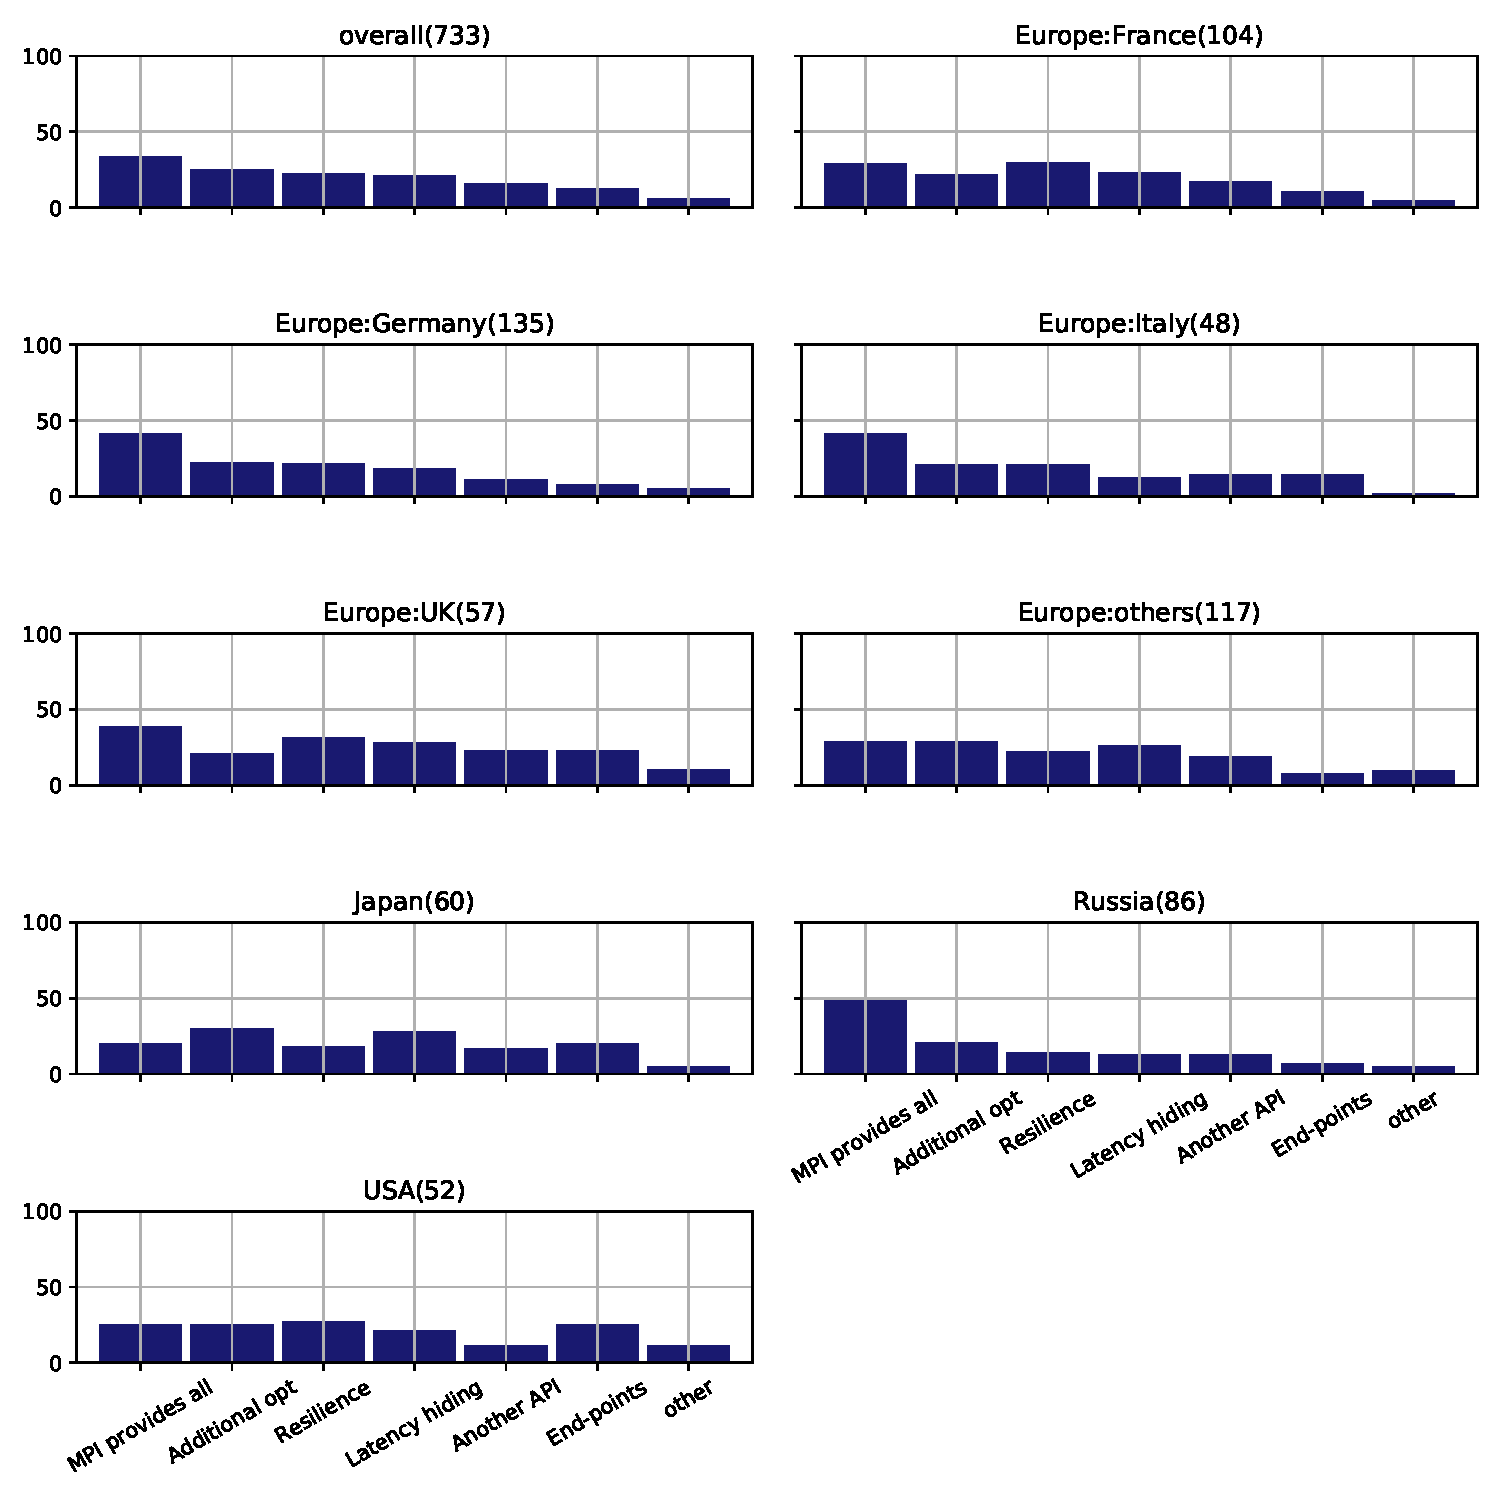
\includegraphics[width=10cm]{../pdfs/Q26.pdf}
\caption{Simple analysis: Q26}
\label{fig:Q26}
\end{center}
\end{figure}
